
% Diese Grundkonfiguration wurde von der Beispielkonfiguration übernommen
\documentclass[12pt,pdftex,parskip=half]{scrartcl}
\usepackage[ngerman]{babel}
\usepackage[utf8]{inputenc}  \usepackage[T1]{fontenc}
\usepackage{graphicx}
\usepackage{xcolor}
\usepackage{pdfpages}
\usepackage{url}


% ändert die Schriftart im gesamten Dokument (nur eine Zeile darf aktiv sein) (Auswahl: http://www.tug.dk/FontCatalogue/)
\usepackage{dejavu}

% hiermit kann das €-Zeichen direkt eingegeben werden
\usepackage{eurosym}  \DeclareUnicodeCharacter{20AC}{\euro}

% Seitenränder
\usepackage{geometry}
\geometry{a4paper,left=20mm,right=20mm,bottom=20mm,top=15mm,bindingoffset=0mm,includehead,includefoot}

% Kopf- und Fußzeile jeweils mit Linie
\usepackage{fancyhdr} \pagestyle{fancy} \renewcommand{\headwidth}{\textwidth}
\renewcommand{\headrulewidth}{0.4pt} \lhead{} \chead{} \rhead{}
\renewcommand{\footrulewidth}{0.4pt} \lfoot{} \cfoot{\small \today} \rfoot{\small \thepage}

% kein Erstzeileneinzug und etwas mehr Zeilenabstand
\setlength{\parindent}{0pt}  \linespread{1.1}

\usepackage[pdftitle={}, pdfauthor={}, pdfstartview=FitH, colorlinks=true, linkcolor=black, urlcolor=blue, citecolor=black]{hyperref}

\usepackage{csquotes}

% Einstellungen für C#-Sourcecode
\usepackage{listings}

\lstset{language=[Sharp]C,
    frame=single,
    basicstyle=\footnotesize\ttfamily,
    breaklines=true,
    breakatwhitespace=false,
    classoffset=1,
    commentstyle=\slshape\color{cyan},
    framextopmargin=2pt,
    framexbottommargin=2pt,
    identifierstyle=\color{violet},
    keywordstyle=\color{yellow},
    morekeywords={main,cin,cout}, keywordstyle=\bfseries\color{magenta},
    rulecolor=\color{black!40},
    showspaces=false, showstringspaces=false,
    stringstyle=\color{blue},
    tabsize=2,
    title=\lstname
}


% Command to insert inline code (Usage: \inlinecode{<language>}{<code>})
\newcommand{\inlinecode}[2]{\colorbox{lightgray}{\lstinline[language=#1]$#2$}}


% Beginn des Textes
\begin{document}


% Deckblatt
\begin{titlepage}
    \begin{center}
        \vfill {{\Large Erstellen einer CDatum Klasse}}
        \vfill {Lernfeld 6: Entwickeln und Bereitstellen von Anwendungssystemen\\Herr Goebel}
        \vfill {von\\Yannick Lapp\\\today}
    \end{center}
\end{titlepage}


% Inhaltsverzeichnis
\tableofcontents
\clearpage


% 1. Aufgabenstellung
\section{Aufgabenstellung}

  % 1.1
  \subsection{Kurze Beschreibung}
  Es sollte eine Datums-Klasse in C\# implementiert werden, die verschiedene Funktionalitäten zum Umgang mit Kalenderdaten bietet.

  C\# ist eine typsichere, objektorientierte Allzweck-Programmiersprache, die von Microsoft entwickelt wurde.
  Mehr Informationen zu C\# können in diesem \href{https://de.wikipedia.org/wiki/C-Sharp}{Wikipedia Artikel} nachgelesen werden.

  Die konkrete Aufgabenstellung befindet sich auf der nächsten Seite.

  \clearpage


  % 1.2
  \subsection{Konkrete Aufgabenstellung}
    \begin{quote}
      \itshape % Make the quote italic
      1.1.1 Erstellen einer Klasse

      Entwerfen und implementieren Sie eine Klasse CDatum. Diese Klasse soll ein Kalenderdatum bestehend aus Tag, Monat und Jahr intern verwalten und an einer von Ihnen festgelegten Schnittstelle die folgenden Funktionalitäten bieten:

      \begin{itemize}
        \item Setzen eines bestimmten Datums
        \item Vergleich zweier Daten (gleich, vorher, nachher)
        \item Addition einer bestimmten Anzahl von Tagen zu einem Datum
        \item Bestimmung der Differenz zwischen zwei Daten im normalen Kalenderjahr
        \item Bestimmung der Differenz zwischen zwei Daten im Bankjahr (360 Tage, jeder Monat 30 Tage)
        \item Berechnung des Wochentages (0-6) eines Datums
        \item Festlegung, ob es sich um einen Feiertag handelt
        \item Erzeugen von Textstrings um das Datum in unterschiedlichen Formaten auszugeben
          (z.B. 2.4.2019, 04.05.2019, 3. Jan 2019, 5. Februar 2019)
        \item Berechung des Julianischen Datums
        \item Gibt es noch weitere Funktionen?
      \end{itemize}

      Schreiben Sie ein Testprogramm, mit dem alle Funktionen dieser Klasse intensiv getestet werden können.
    \end{quote}

    \clearpage


% 2. Grober Überblick
\section{Überblick über die umgesetzte Klasse}

    % 2.1
    \subsection{Quellcode}

    Der Quellcode für die Klasse und das Testprogramm kann in diesem git repository eingesehen werden:\\
    \href{https://github.com/ylapp1/CDate}{https://github.com/ylapp1/CDate}

    Um die Übersichtlichkeit zu erhöhen wurden neben der Klasse "`CDate"' auch noch einige Hilfsklassen implementiert, die die "`CDate"' Klasse dabei unterstützen, ihre Aufgabe zu erfüllen.

    Der Quellcode ist in Englisch geschrieben.
    Im Code befinden sich auch Kommentare auf Englisch, die Funktionen, Klassen und manche Code Schnipsel näher beschreiben.

    In den folgenden Kapiteln wird die Funktion der einzelnen Dateien sowie die damit umgesetzte Lösung der Aufgaben erklärt.


    % 2.2
    \subsection{Anforderungen}
    Das Paket "`mono-mcs"' muss installiert sein.\\
    Dann kann das Test-Programm mit dem "`compile.sh"' Skript kompiliert werden.
    Das Ergebnis ist die ausführbare Datei "`check"'.

    \clearpage


% 3
\section{Funktionen der einzelnen Dateien}

    % 3.1
    \subsection{/}
    Das Hauptverzeichnis beinhaltet das Test-Programm, das die Funktionalitäten der Klasse testet.

      % 3.1.1
      \subsubsection{.gitignore}
      Da das Projekt in einem git Repository liegt gibt es auch eine .gitignore Datei, die Muster in Dateipfaden definiert, die von git ignoriert werden sollen. In diesem Fall sind das die von doxygen generierten Dateien sowie die aus dem Code kompilierbare ausführbare Datei.

      % 3.1.2
      \subsubsection{Doxyfile}
      Hierin ist die Konfiguration abgelegt, mithilfe der das Programm \href{http://www.doxygen.nl/}{doxygen} aus den Kommentaren im Quellcode eine Entwickler-Dokumentation generieren kann.
      Dazu wird im Hauptverzeichnis des Repositorys einfach der Befehl \inlinecode{bash}{doxygen} ausgeführt, das Programm sucht und findet die Datei "`Doxyfile"' dann von alleine und wendet die Konfiguration an.


      Diese Konfigurationsdatei wurde mit \inlinecode{bash}{doxygen -g} generiert und hat die meisten Einstellungen bei den Standardwerten belassen, die folgenden Konfigurationswerte wurden tatsächlich geändert:

        \begin{itemize}
          \item PROJECT\_NAME: ``CDatum''
          \item OUTPUT\_DIRECTORY: ``docs/doxygen''
          \item OUTPUT\_LANGUAGE: ``German''
          \item EXTRACT\_*: Alle ``YES''
          \item INPUT: ``src''
          \item RECURSIVE: ``YES''
        \end{itemize}

      % 3.1.3
      \subsubsection{README.md}
      Eine kurze Beschreibung des Projekts und ein paar Dinge, die nützlich zu wissen sind in Bezug auf das Projekt.

      % 3.1.4
      \subsubsection{check-functionality.c}
      Der Quelltext des Test-Programms, das die Funktionalität der entwickelten Klassen überprüft.

      % 3.1.5
      \subsubsection{compile.sh}
      Ein shell Skript, mit dem das Test-Programm kompiliert werden kann. Dieses Skript generiert eine ausführbare Datei names ``check''. Diese kann dann mit \inlinecode{bash}{./check} ausgeführt werden.
      Das Skript ist nur unter Linux ausführbar.

      \clearpage


    % 3.2
    \subsection{/docs}

    Beinhaltet die Dateien, die zum Generieren der Dokumentation erforderlich sind.
    Dazu zählen die Latex Datei Dokumentation.tex sowie Dateien, die von dem Latex Dokument eingebunden werden, wie etwa die von doxygen erzeugte PDF Datei.

    \clearpage


    % 3.3
    \subsection{/src}
    Beinhaltet die entwickelten Klassen, darunter auch die CDate Klasse.


      % 3.3.1
      \subsubsection{/}
      Beinhaltet die CDate Klasse und die CDateDiff Klasse. Die CDate Klasse ist die einzige Klasse, die direkt benutzt werden sollte, alle anderen Klassen sind nur dazu gut, um dieser Klasse zu "`helfen"', ihre Funktion zu erfüllen.

        \paragraph{CDate}
        Die Klasse, die im Rahmen der Aufgabenstellung entwickelt werden sollte.
        Sie bietet einige nützliche Funktionen für Kalenderdaten.

        \paragraph{CDateDiff}
        Eine Klasse, die die Differenz zwischen zwei CDate's speichert (in Tagen, Monaten und Jahren).


      % 3.3.2
      \subsubsection{Calendar}
      Beinhaltet Klassen, die zurückgeben können, wie viele Tage ein Monat in einem bestimmten Jahr hat.

        \paragraph{CCalendar}
        Abstrakte Basis-Klasse, die vorgibt, welche Methoden die Unterklassen implementieren müssen

        \paragraph{CCalendar360}
        Ein Kalender, der für jeden Monat in jedem Jahr eine Anzahl von 30 Tagen zurückgibt

        \paragraph{CCalendarNormal}
        Ein Kalender, der dem gebräuchlichen 365 Tage Kalender entspricht.

      \clearpage


      % 3.3.3
      \subsubsection{Holidays}
      Beinhaltet Klassen, die zurückgeben können, welcher Feiertag an einem bestimmten Datum ist.

        \paragraph{OfficialHolidays}
        Abstrakte Basis-Klasse, die vorgibt, welche Methoden die Unterklassen implementieren müssen

        \paragraph{GermanyOfficialHolidays}
        Klasse, die alle Feiertage aus Deutschland kennt, sie unterscheidet aber nicht zwischen Bundesländern

      % 3.3.4
      \subsubsection{Util}
      Beinhaltet sonstige Hilfsklassen.

        \paragraph{MonthInfo}
        Kann Informationen über einen Monat zurückgeben (dazu zählt der komplette und der abgekürzte Name)

  \clearpage


% 4
\section{Lösung der Aufgabenstellungen}

  % 4.1
  \subsection{Setzen eines bestimmten Datums}

  \begin{lstlisting}
      /**
       * CDate constructor.
       *
       * @param _day The day number
       * @param _month The month number
       * @param _year The year number
       *
       * @throws Exception The Exception when the specified date is invalid
       */
      public CDate(int _day, int _month, int _year)
      {
        validateDate(_day - 1, _month - 1, _year);

        day = _day - 1;
        month = _month - 1;
        year = _year;
      }
  \end{lstlisting}

  Ein Konstruktor der CDate Klasse akzeptiert als Parameter "`Tag"', "`Monat"' und "`Jahr"'.
  Dann setzt er die internen Attribute "`Tag"', "`Monat"' und "`Jahr"' enstprechend.

  \clearpage


  % 4.2
  \subsection{Vergleich zweier Daten (gleich, vorher, nachher)}

  \begin{lstlisting}
      /**
       * Returns the comparison status to a different CDate.
       *
       * @param _otherDate The comparison date
       *
       * @return int The comparison status (one of the COMPARESTATUS_* constants)
       */
      public int compareTo(CDate _otherDate)
      {
        int yearDiff = _otherDate.year - year;
        if (yearDiff == 0)
        { // The year number is the same, check the month

          int monthDiff = _otherDate.month - month;
          if (monthDiff == 0)
          { // The month number is the same, check the day

            // Math.Sign returns the sign of the number (-1 = -, 0 = 0, +1 = +)
            int dayDiff = _otherDate.day - day;
            return Math.Sign(dayDiff);
          }
          else return Math.Sign(monthDiff);
        }
        else return Math.Sign(yearDiff);
      }
  \end{lstlisting}


  Es wurde die Methode "`compareTo"' hinzugefügt, die als Parameter ein anderes CDate akzeptiert und den Vergleichs-Status zurückgibt.

  Dazu wurden der Klasse CDate drei Konstanten hinzugefügt, die von der Methode zurückgegeben werden können:
    \begin{itemize}
      \item COMPARESTATUS\_LOWER\_THAN\_COMPARISON\_DATE: Das verglichene Datum ist größer
      \item COMPARESTATUS\_EQUAL\_TO\_COMPARISON\_DATE: Das verglichene Datum ist gleich
      \item COMPARESTATUS\_HIGHER\_THAN\_COMPARISON\_DATE: Das verglichene Datum ist niedriger
    \end{itemize}

    Die Werte der Konstanten entsprechen dabei den möglichen Rückgabewerten von \inlinecode{C}{Math.Sign}.


  \clearpage


  % 4.3
  \subsection{Addition einer bestimmten Anzahl von Tagen zu einem Datum}

  \begin{lstlisting}
    /**
     * Adds a number of days to this CDate.
     *
     * @param _numberOfDays The number of days to add
     */
    public void addDays(int _numberOfDays)
    {
      day = day + _numberOfDays;

      int numberOfDaysExceededForMonth;
      do
      {
        numberOfDaysExceededForMonth = getNumberOfDaysExceededForMonthInCalendar(calendarNormal);
        if (numberOfDaysExceededForMonth > 0)
        {
          day = numberOfDaysExceededForMonth;
          addMonths(1);
        }
      }
      while (numberOfDaysExceededForMonth > 0);
    }

    /**
     * Adds a number of months to this CDate.
     *
     * @param _numberOfMonths The number of months to add
     */
    private void addMonths(int _numberOfMonths)
    {
      month += _numberOfMonths;

      year += (int)(month / 12);
      month = month % 12;
    }
  \end{lstlisting}


  Es wurde die Methode "`addDays"' hinzugefügt, die als Parameter eine Anzahl von Tagen entgegennimmt.
  Intern rechnet sie dann Monat für Monat hoch, solange die Anzahl Tage höher ist als die Anzahl Tage in dem aktuellen Monat des Datums. Nebenbei wird auch das Jahr erhöht, falls dadurch der 12. Monat überschritten wird.
  Der Referenzkalender ist hierbei immer der normale Kalender mit 365 Tagen.

  \clearpage


  % 4.4
  \subsection{Bestimmung der Differenz zwischen zwei Daten im normalen Kalenderjahr}

  \begin{lstlisting}
      /**
       * Returns the difference to another date using the regular calendar.
       *
       * @param _otherDate The date to compare this date to
       *
       * @return CDateDiff The difference to the other date
       */
       public CDateDiff diffNormal(CDate _otherDate)
       {
         return diff(_otherDate, calendarNormal);
       }
  \end{lstlisting}


  Es wurde die Methode "`diffNormal"' hinzugefügt, die ein anderes CDate als Parameter akzeptiert und ein CDateDiff zurückgibt, in dem die genaue Differenz in Tagen, Monaten und Jahren gespeichert ist.

  Um Code Duplizierung zu vermeiden verwendet "`diffNormal"' intern diesselbe Methode wie die Methode für die Differenz zweier Daten im Bankjahr.
  Dies ist durch die Verwendung der "`CCalendar"' Klassen möglich, die zurückgeben, wie viele Tage ein Monat in einem bestimmten Jahr hat.

    \clearpage


    % 4.4.1
    % The label is used to reference this subsubsection in the next subsection
    \subsubsection{Allgemeine Differenzberechnung} \label{4.4.1}
    \begin{lstlisting}
        /**
         * Calculates and returns the difference to another date in a specified calendar.
         *
         * @param _otherDate The date to compare this date to
         * @param _calendar The calendar to use for the comparison
         *
         * @return CDateDiff The difference to the other date
         */
        private CDateDiff diff(CDate _otherDate, CCalendar _calendar)
        {
          // Base date is the lower one
          bool isNegativeDiff;
          CDate lowerDate;
          CDate higherDate;

          if (compareTo(_otherDate) == COMPARESTATUS_LOWER_THAN_COMPARISON_DATE)
          {
            lowerDate = this;
            higherDate = _otherDate;
            isNegativeDiff = true;
          }
          else
          { // Equal or bigger than comparison date
            lowerDate = _otherDate;
            higherDate = this;
            isNegativeDiff = false;
          }


          int yearDiff = higherDate.year - lowerDate.year;
          int monthDiff = higherDate.month - lowerDate.month;
          int dayDiff = higherDate.day - lowerDate.day;

          int targetMonth, targetYear, monthOffset = 0;

          // Normalize days
          while (dayDiff < 0)
          {
            monthDiff -= 1;

            targetMonth = lowerDate.monthNumber() + (monthOffset % 12);
            targetYear = lowerDate.year + (int)(monthOffset / 12);

            dayDiff += _calendar.getNumberOfDaysInMonth(targetMonth, targetYear);
            monthOffset++;
          }

          while (monthDiff < 0)
          {
            yearDiff -= 1;
            monthDiff += 12;
          }

          return new CDateDiff(isNegativeDiff, dayDiff, monthDiff, yearDiff);
        }
    \end{lstlisting}

    Diese interne Methode nimmt einen CCalendar sowie ein zu vergleichendes CDate entgegen und berechnet die Differenz in folgenden Schritten:

    \begin{enumerate}
      \item Herausfinden, welches Datum das niedrigere ist (mit Hilfe von "`compareTo"')
      \item Differenz zwischen Jahr, Monat und Tag ausrechnen
      \item Tage solange um die Anzahl Tage des aktuellen Monats erhöhen bis die Anzahl Tage nicht mehr kleiner als 0 ist, für jede Erhöhung wird die Anzahl Monate in der Differenz um 1 verringert
      \item Monate solange um 12 erhöhen bis die Anzahl Monate nicht mehr kleiner als 0 ist, für jede Erhöhung wird die Anzahl Jahre um 1 verringert
    \end{enumerate}

    \clearpage


    % 4.5
    \subsection{Bestimmung der Differenz zwischen zwei Daten im Bankjahr (360 Tage, jeder Monat 30 Tage)}

    \begin{lstlisting}
        /**
         * Returns the difference to another date using the bank calendar.
         *
         * @param _otherDate The date to compare this date to
         *
         * @return CDateDiff The difference to the other date
         */
        public CDateDiff diff360(CDate _otherDate)
        {
          return diff(_otherDate, calendar360);
        }
    \end{lstlisting}

    Es wurde die Methode "`diff360"' hinzugefügt, die intern die selbe Methode wie "`diffNormal"' verwendet.
    Statt dem normalen Kalender übergibt sie aber den "`Calendar360"'.

    Die Funktionsweise der internen Methode kann in \hyperref[4.4.1]{\color{blue}Abschnitt 4.4.1} nachgelesen werden.

    \clearpage


    % 4.6
    \subsection{Berechnung des Wochentages (0-6) eines Datums}

    \begin{lstlisting}
      /**
       * Returns the day of the week of this date.
       *
       * @return int The day of the week
       */
      public int getDayOfWeek()
      {
        int century = (int)(year / 100);
        int yearOfCentury = year % 100;

        int dayNumber = day + 1;

        // 1 = March, 2 = April, ...
        int monthNumber = (month - 2) + 1;
        while (monthNumber < 0) monthNumber += 12;

        /*
         * This formula was taken from https://de.wikipedia.org/wiki/Wochentagsberechnung#4._Allgemeing%C3%BCltige_Formel and
         * https://cs.uwaterloo.ca/~alopez-o/math-faq/node73.html
         */
        int weekDayNumber = (dayNumber + (int)(2.6 * monthNumber - 0.2) + yearOfCentury + (int)(yearOfCentury / 4) + (int)(century / 4) - 2 * century) % 7;

        return weekDayNumber - 1;
      }
    \end{lstlisting}

    Es wurde die Methode "`getDayOfWeek"' hinzugefügt.
    Diese berechnet mit Hilfe einer Formel den Wochentag des Datums, und gibt den Wert um eins verringert zurück, um der Anforderung "`Berechnung des Wochentages (0-6)"' gerecht zu werden.

    \clearpage


    % 4.7
    \subsection{Festlegung, ob es sich um einen Feiertag handelt}

    \begin{lstlisting}
        /**
         * Returns whether this date is an official holiday.
         *
         * @return bool True if this date is an official holiday, false otherwise
         */
        public bool isOfficialHoliday()
        {
          return !String.Equals(germanyHolidays.getDayOfficialHolidayName(this), "");
        }
    \end{lstlisting}

    Es wurde eine allgemeine "`OfficialHolidays"' Klasse hinzugefügt, und anschließend eine "`GermanyOfficialHolidays"' Klasse davon abgeleitet, die alle Feiertage aus Deutschland (unabhängig vom Bundesland) kennt.\\
    Mit Hilfe der Methode "`getDayOfficialHolidayName"' kann überprüft werden, ob ein Tag ein Feiertag ist. Gibt die Methode den Namen eines Feiertags zurück, so ist der Tag ein Feiertag. Gibt sie allerdings einen leeren String zurück ist der Tag kein Feiertag.

    Zur Lösung der Aufgabe wurde die Methode "`isOfficialHoliday"' zur CDate Klasse hinzugefügt, die intern diese Logik befolgt.

    \clearpage


    % 4.8
    \subsection{Erzeugen von Textstrings um das Datum in unterschiedlichen Formaten auszugeben (z.B. 2.4.2019, 04.05.2019, 3. Jan 2019, 5. Februar 2019)}

    \begin{lstlisting}
        /**
         * Returns this date as a formatted string.
         *
         * The following format specifiers are available:
         * - %d = day number
         * - %m = month number
         * - %y = year number
         * - %F = full month name
         * - %M = short month name
         *
         * You may add ":<zeroes>.<zeros>" to define by how many zeros the numbers must be padded (usage is the same as in String.Format output variable specifiers).
         *
         * @param _formatString The format string
         *
         * @return string The formatted date string
         */
        public string toFormattedString(string _formatString)
        {
          string formatString = Regex.Replace(_formatString, "%d:(\\d+)", "{0:$1}");
          formatString = Regex.Replace(formatString, "%m:(\\d+)", "{1:$1}");
          formatString = Regex.Replace(formatString, "%y:(\\d+)", "{2:$1}");

          MonthInfo monthInfo = new MonthInfo(monthNumber());
          if (formatString.Contains("%F"))
          { // Full month name
            formatString = formatString.Replace("%F", monthInfo.getFullName());
          }
          if (formatString.Contains("%M"))
          { // Short month name
            formatString = formatString.Replace("%M", monthInfo.getShortName());
          }

          formatString = formatString.Replace("%d", "{0}").Replace("%m", "{1}").Replace("%y", "{2}");

          return String.Format(formatString, dayNumber(), monthNumber(), year);
        }
    \end{lstlisting}

    \clearpage

    Es wurde eine Methode "`toFormattedString"' hinzugefügt, die den Datums-String mithilfe sogenannter "`Format-Specifier"' generiert.
    Um alle Beispiele möglich zu machen waren diese specifier nötig:

      \begin{itemize}
        \item \%d: Die Nummer des Tages
        \item \%m: Die Nummer des Monats
        \item \%y: Die Nummer des Jahres
        \item \%F: Vollständiger Monatsname
        \item \%M: Abgekürzter Monatsname
      \end{itemize}

      An die "`Nummer"' specifier können auch "`:<Nullen>.<Nullen>"' angehängt werden, um die Zahlen mit führenden Nullen aufzufüllen. Das Format entspricht dabei den Formaten, die bei einzufügenden Variablen in \inlinecode{C}{String.Format} kompatiblen Strings verwendet werden können.

      \clearpage


      % 4.9
      \subsection{Berechung des Julianischen Datums}

      \begin{lstlisting}
        /**
         * Returns the julian date that equals this gregorian date.
         * Using the algorithm from here: https://de.wikipedia.org/wiki/Julianisches_Datum#Umrechnung_Kalenderdatum_%E2%86%92_JD
         *
         * @return double The julian date
         */
        public double toJulianDate()
        {
          int y, m;
          if (monthNumber() > 2)
          {
            y = year;
            m = monthNumber();
          }
          else
          {
            y = year - 1;
            m = monthNumber() + 12;
          }

          int d = dayNumber();
          int b = 2 - (int)Math.Floor((double)(y / 100)) + (int)Math.Floor((double)(y / 400));

          return Math.Floor((double)(365.25 * (y + 4716))) + Math.Floor((double)(30.6001 * (m + 1))) + d + b - 1524.5;
        }
      \end{lstlisting}

      Es wurde eine Methode "`toJulianDate"' hinzugefügt, die mit Hilfe einer Formel das dem CDate entsprechende julianische Datum errechnet und zurückgibt.

      \clearpage


      % 4.10
      \subsection{Gibt es noch weitere Funktionen?}

        % 4.10.1
        \subsubsection{toString}

        \begin{lstlisting}
          /**
           * Returns this date as a string in the format "DD.MM.YYYY".
           *
           * @return string This date as a string
           */
          public string toString()
          {
            return String.Format("{0:00}.{1:00}.{2:0000}", day + 1, month + 1, year);
          }
        \end{lstlisting}

        Die Methode "`toString"' gibt einen String im Format "`DD.MM.YYYY"' zurück, in dem das in einem CDate gespeicherte Datum enthalten ist.
        Diese Methode wurde noch vor Implementierung der "`toFormattedString"' Methode hinzugefügt.

        \clearpage


        % 4.10.2
        \subsubsection{Validierung}

        \begin{lstlisting}
            /**
             * Validates a date.
             *
             * @param _day The day number (0 - 30)
             * @param _month The month number (0 = January, 11 = December)
             * @param _year The year number
             *
             * @throws Exception The Exception when the specified date is invalid
             */
            private void validateDate(int _day, int _month, int _year)
            {
              if (_month < 0 || _month > 11) throw new Exception("Invalid month");
              else if (_day < 0) throw new Exception("Invalid day");
              else if (getNumberOfDaysExceededForMonthInCalendar(calendarNormal) > 0 && getNumberOfDaysExceededForMonthInCalendar(calendar360) > 0)
              {
                throw new Exception("This day is invalid for that month in all supported calendar types");
              }
            }
        \end{lstlisting}

        Das im Konstruktor übergebene Datum wird validiert und falls es weder im Bank-Kalender noch im "`normalen"' Kalender ein solches Datum gibt wird eine Exception geworfen. Das sorgt für den Abbruch des Programms falls die Ausnahme nicht behandelt wird.

        \clearpage


% 5
\section{Testen der umgesetzen Klasse}

Die Aufgabenstellung beinhaltete auch, dass ein Testprogramm, mit dem alle Funktionen der Klasse intensiv getestet werden können, implementiert werden soll.

Dazu wurde eine Klasse "`Program"' mit einer statischen "`Main"' Methode implementiert, die die Tests durchführt. Diese Klasse hat einige Hilfsmethoden, die sich an Methoden von "`Unit Test"' Frameworks orientieren. Dazu zählen:

  \begin{itemize}
    \item assertStringEquals: Prüft, dass zwei strings gleich sind, falls nicht wird das Programm mit einem Fehler beendet
    \item assertIntEquals: Prüft, dass zwei integers gleich sind, falls nicht wird das Programm mit einem Fehler beendet
    \item assertBoolEquals: Prüft, dass zwei booleans gleich sind, falls nicht wird das Programm mit einem Fehler beendet
  \end{itemize}

Um die Übersichtlichkeit zu gewährleisten wurde für jede Aufgabenstellung eine eigene statische Methode hinzugefügt, die die entsprechende Funktionalität testet.
Die Umsetzung der Tests wird im Folgenden beschrieben.


  % 5.1
  \subsection{Setzen eines bestimmten Datums}
  Es wurden ein paar CDate's instanziert und anschließend überprüft, dass die "`toString"' Methode den erwarteten Datums-String zurückgibt.

  % 5.2
  \subsection{Vergleich zweier Daten (gleich, vorher, nachher)}
  Es wurden CDate Paare instanziert und anschließend mit der "`compareTo"' Methode verglichen. Dabei wurde geprüft, dass der zurückgegebene Wert der erwarteten COMPARESTATUS Konstante entspricht.

  % 5.3
  \subsection{Addition einer bestimmten Anzahl von Tagen zu einem Datum}
  Es wurden ein paar CDate's instanziert und dazu Tage addiert, einmal mit Monatsüberlauf und einmal ohne und es wurde geprüft, dass das Datum zum erwarteten Datum umgewandelt wurde.

  % 5.4
  \subsection{Bestimmung der Differenz zwischen zwei Daten im normalen Kalenderjahr}
  Es wurden ein paar CDate Paare instanziert und mit "`diffNormal"' verglichen. Dabei wurde geprüft, dass die Differenz der erwarteten Differenz entspricht.

  % 5.5
  \subsection{Bestimmung der Differenz zwischen zwei Daten im Bankjahr (360 Tage, jeder Monat 30 Tage)}
  Es wurde ein CDate Paar instanziert und mit "`diff360"' verglichen. Dabei wurde geprüft, dass die Differenz der erwarteten Differenz entspricht.

  % 5.6
  \subsection{Berechnung des Wochentages (0-6) eines Datums}
  Es wurden einige CDate's instanziert mit Daten von denen der Wochentag bereits im Vorhinein bekannt war. Dann wurde geprüft, dass die Methode "`getDayOfWeek"' die Nummer des erwarteten Wochentages zurückgibt.

  % 5.7
  \subsection{Festlegung, ob es sich um einen Feiertag handelt}
  Es wurde für das komplette Jahr 2019 für jeden deutschen Feiertag geprüft, dass dieser von CDate als Feiertag erkannt wird.
  Außerdem wurde bei ein paar Tagen, die keine Feiertage sind, geprüft, dass CDate diese nicht als Feiertag erkennt.

  % 5.8
  \subsection{Erzeugen von Textstrings um das Datum in unterschiedlichen Formaten auszugeben (z.B. 2.4.2019, 04.05.2019, 3. Jan 2019, 5. Februar 2019)}
  Es wurden ein paar Beispiel-Strings aus CDate's generiert und geprüft, dass das Ergebnis dem erwarteten string entspricht.
  Die getesteten  Beispiele beinhalten sämtliche Format specifier, die unterstützt werden.


  % 5.9
  \subsection{Berechung des Julianischen Datums}
  Es wurden ein paar CDate's instanziert für Kalenderdaten von denen das entsprechende julianische Datum vorher durch ein Online-Tool berechnet wurde. Dann wurde geprüft, dass das Ergebnis von "`toJulianDate"' dem erwarteten julianischen Datum entspricht.

  \clearpage



% 6
\section{Ausblick und Ideen}

Die entwickelte CDate Klasse zielt darauf ab, die Anforderungen der Aufgabenstellung zu erfüllen.
Dennoch gibt es noch ein paar Ideen, die umgesetzt werden könnten sowie ein paar Einschränkungen der aktuellen Lösung.

  % 6.1
  \subsection{Einschränkungen}

    \begin{itemize}
      \item Die Methode CDate::isOfficialHoliday() verwendet immer GermanyOfficialHolidays, man kann also nie Feiertage für andere Länder prüfen
      \item Die Klasse GermanyOfficialHolidays bietet keine Möglichkeit zu unterscheiden, in welchem Bundesland der jeweilige Feiertag tatsächlich gilt
      \item Kurze und volle Monatsnamen sind hardgecoded auf deutsche Monatsnamen
      \item CDate::addDays verwendet immer CalendarNormal als Referenzkalender
    \end{itemize}


  \subsection{Mögliche Verbesserungen}

    \begin{itemize}
      \item CDate Konstruktor hinzufügen, der Format und Datums-String entgegennimmt und Tag, Monat und Jahr aus dem String parsed
      \item CDate Konstruktor hinzufügen, der ein julianisches Datum entgegennimmt und daraus das entsprechende Datum des gregorianischen Kalenders errechnet
      \item Die Tests könnten noch ausführlicher sein, insbesondere die Tests für "`compareTo"' und "`addDays"'
    \end{itemize}

  \clearpage


% 7
\section{Doxygen Dokumentation}

Auf den nachfolgenden Seiten befindet sich die gesamte von doxygen generierte Dokumentation für die CDate Klasse und ihre Hilfsklassen.

  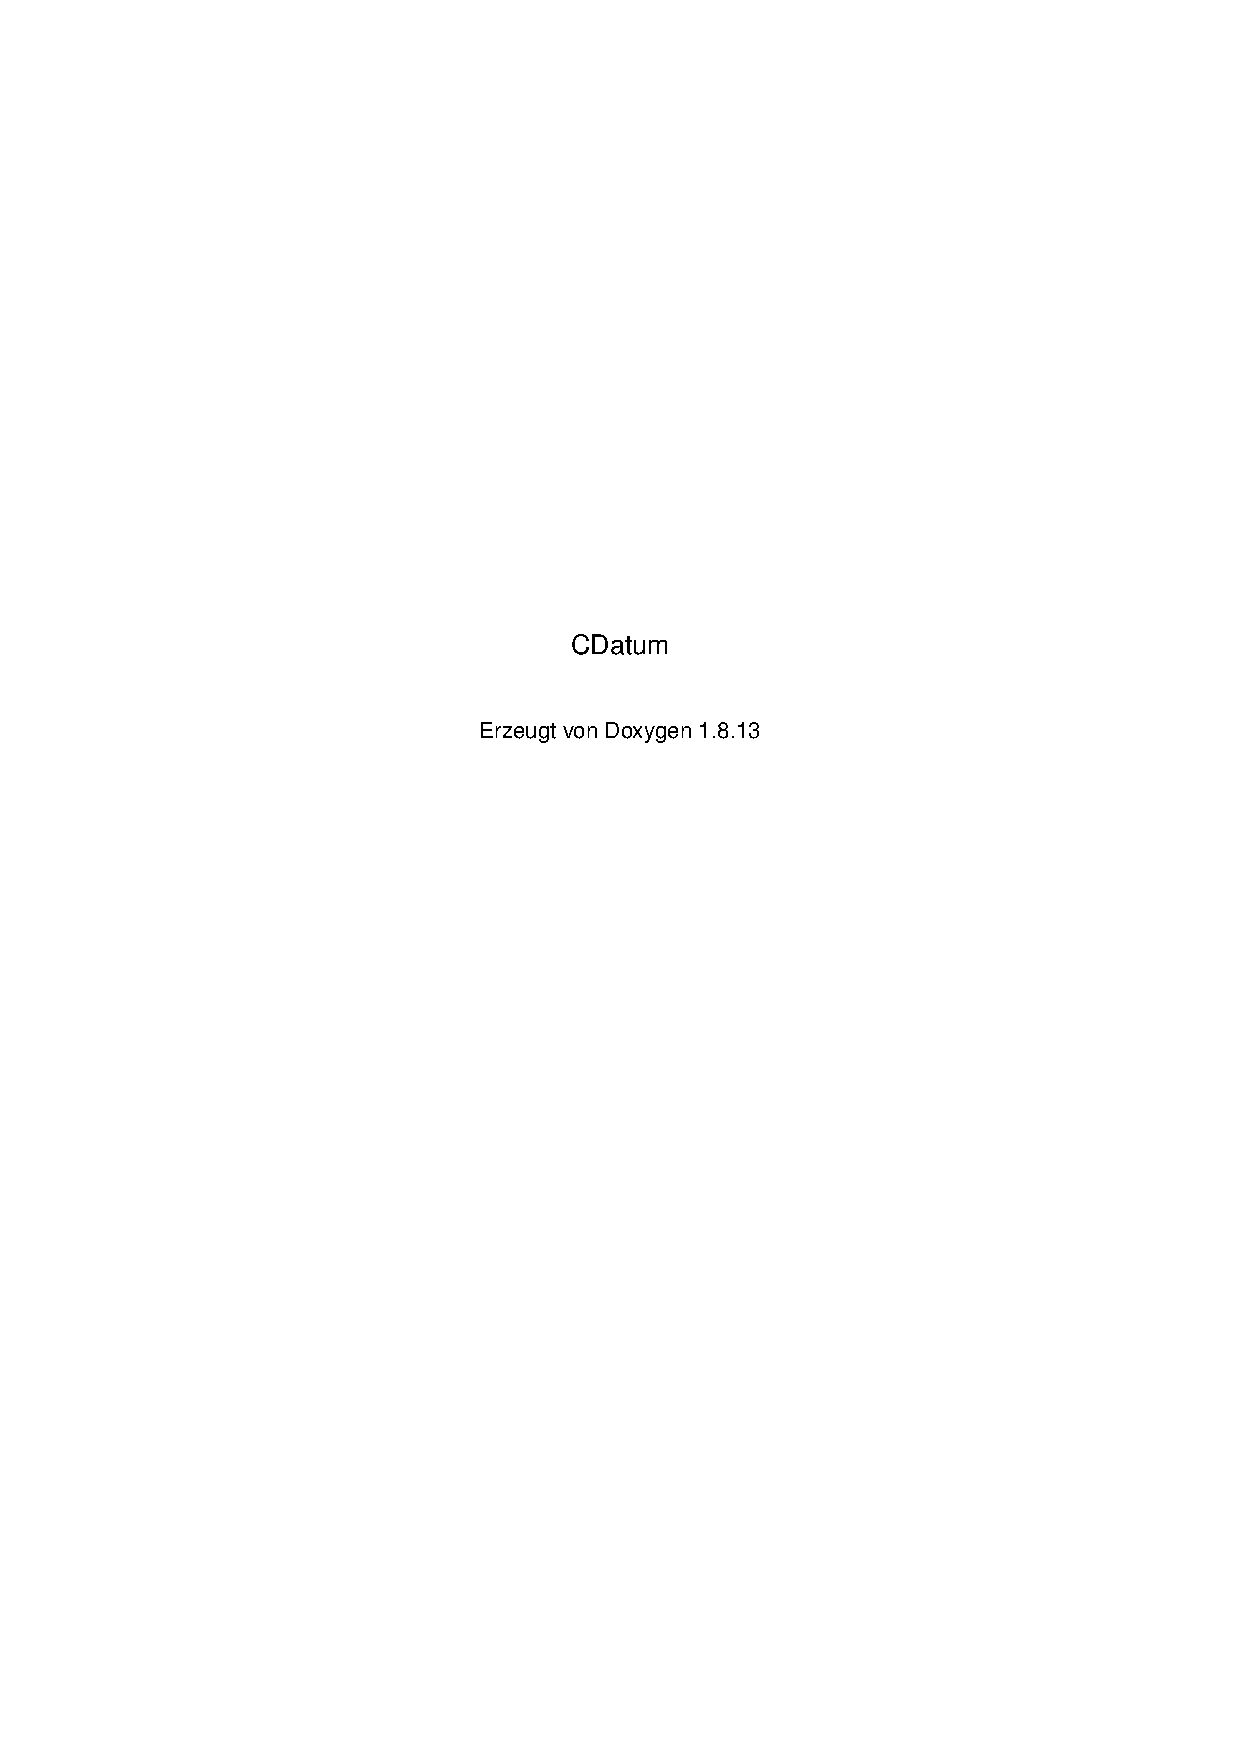
\includepdf[scale=0.9,frame=true,pages=-]{refman}

\end{document}
